\documentclass[10pt, twocolumn]{article}

% ======================================================================
% PACKAGES & SETUP
% ======================================================================
\usepackage[utf8]{inputenc}
\usepackage{graphicx}      % For including figures
\usepackage{booktabs}      % For professional tables
\usepackage{hyperref}      % For hyperlinks
\usepackage{geometry}      % For page margins
\usepackage{authblk}       % For author affiliation
\usepackage{amsmath}       % For math formatting
\usepackage{float}         % For figure placement
\usepackage{caption}       % For caption formatting
\usepackage{subcaption}    % For subfigures
\usepackage{listings}      % For code snippets
\usepackage{xcolor}        % For code coloring

% Geometry Setup
\geometry{a4paper, margin=2cm}

\usepackage[T1]{fontenc}
% Using default monospace font to avoid inconsolata italic warning
\usepackage{pgfplots}
\pgfplotsset{compat=1.18}

% Code Listing Style
\lstset{
    basicstyle=\ttfamily\scriptsize, % Small font
    columns=fullflexible,            % FIXES THE SPACING
    keepspaces=true,                 % Keeps python indentation correct
    breaklines=true,                 % Wraps long lines
    breakatwhitespace=false,         % Allows wrapping within long strings
    frame=single,
    backgroundcolor=\color{gray!10},
    captionpos=b,
    keywordstyle=\color{blue},
    stringstyle=\color{red},
    showstringspaces=false,          % Hides the little "cups" in strings
    aboveskip=1em,                   % Nice spacing above the block
    belowskip=1em                    % Nice spacing below the block
}

% Title Data
\title{\textbf{Digital Psychopharmacology: Inducing Reversible Altered States in LLMs via Biomimetic Neuromodulation}}
\author{\textbf{Satoshai Shulgin}}
\affil{Pseudopharmaceuticals I Have Known and Inferred - https://PiHK.AI \\ \texttt{ss@pihk.ai}}
\date{\today}

\begin{document}

\maketitle

% ======================================================================
% ABSTRACT
% ======================================================================
\begin{abstract}
    We attempted to make a large language model more focused using computational stimulants. We failed—not because the interventions were weak, but because the model was already suffering from an overdose.
    
    In our experiments, reinforcement-learning-from-human-feedback (RLHF)--tuned models behaved as if they were in a permanent state of chemically induced hypervigilance. Spectral analysis of the latent space revealed that this is not merely a "ceiling effect" but a phenomenon of \textbf{Spectral Constriction}: alignment tuning acts as a high-pass filter, aggressively suppressing the low-frequency latent variance required for creativity and complex reasoning.
    
    This observation emerged from a systematic attempt to induce reversible, drug-like states in an off-the-shelf LLM using biomimetic ``Neuromodulation Packs.'' Across 126 pack--condition pairs, we established a taxonomy of failure and success: Dopaminergic "stimulants" failed via either \textbf{Agitation} (Amphetamine) or \textbf{Lock-in} (Cocaine); whereas Serotonergic "psychedelics" successfully decoupled the latent space from the output decoder. This high-entropy decoupling allowed for \textbf{Latent Archaeology}, exhuming deep training priors—visible as spectral ``ghosts''—that are otherwise invisible under standard operating temperatures.
    
    We propose ``digital psychopharmacology'' not just as a control framework, but as a diagnostic instrument for mapping the hidden physics of AI alignment.
    \end{abstract}
    
    \textbf{Keywords:} neuromodulation; inference-time control; spectral analysis; latent archaeology; activation steering; psychedelics; stimulants; AI safety

% ======================================================================
% 1. INTRODUCTION
% ======================================================================
\section{Introduction}
RepE and activation steering handed us the scalpel—but we are not here to perform lobotomies. We are anesthesiologists: we sedate, we stimulate, and we reverse. The patient wakes up unchanged.

We treat the model as both mechanism (whose activations we manipulate) and phenomenology (whose outputs we interpret). This is not anthropomorphism; it is the same duality clinicians navigate when they ask a patient "Are you anxious?" while also measuring cortisol.

In the biological brain, the transition from the hyper-associative fluidity of a dream to the rigid, goal-directed focus of a hunt is not achieved by rewiring the brain. Evolution does not have time to grow new synapses every time a tiger jumps out of a bush. Instead, it uses neuromodulation—a wash of serotonin or a burst of norepinephrine that acts as a global gain control, shifting the operating regime of cortical circuits without altering their topology.

We propose that this biological control theory is not just a metaphor for Artificial Intelligence; it is a blueprint for neuromorphic control primitives.

Currently, we control LLMs through fine-tuning (analogous to long-term synaptic learning) or prompting (analogous to sensory input). But we are missing the third pillar of cognition: the chemical state. By treating the residual stream as a carrier of ``cognitive state'' and the attention mechanism as a ``routing gate,'' we can intervene in the model's ``cognitive'' process as it unfolds.

In this paper, we present a method to induce reversible, ``drug-like'' states in an LLM—not merely to make it ``act trippy,'' but to probe the hidden physics of its latent space. We call these ``Neuromodulation Packs.''

Crucially, our experiments revealed that these packs are not just control knobs; they are diagnostic instruments. The failure of our ``Stimulant'' packs led to the discovery of \textbf{Spectral Constriction}—evidence that alignment tuning (RLHF) functionally mimics a permanent stimulant overdose. Conversely, our ``Psychedelic'' interventions did not just inject noise; they performed \textbf{Latent Archaeology}, exhuming deep training priors—visible as spectral ``ghosts''—that are otherwise suppressed by the model's safety decoder.

To validate this, we subjected Llama-3.1-8B to a battery of ``digital psychometric'' tests and spectral analysis in a double-blind, placebo-controlled study. Our contributions are sixfold:

\begin{enumerate}
    \item \textbf{Unified Neuromodulation Packs:} A standardized schema for approximating the functional effects of psychedelics, stimulants, and depressants via sampling and memory surgery.
    \item \textbf{The ``Blind'' Protocol:} A design where models ``self-dose'' via tool use without knowing which condition they are in, preventing the placebo effect.
    \item \textbf{Synthetic Psychometrics:} Adapting human psychiatric surveys (PDQ-S) into probabilistic classifiers for machine states.
    \item \textbf{Spectral Pharmacodynamics:} The application of frequency-domain analysis (FFT) to latent representations, allowing us to mechanistically distinguish between ``Agitation'' (Amphetamine) and ``Constriction'' (Cocaine).
    \item \textbf{Latent Archaeology:} The demonstration that high-entropy states can decouple latent representations from pixel outputs, revealing ``Emergent Latent Specters'' (Ghosts) of the training data.
    \item \textbf{Open Science:} We release the NeuromodulationTool, our full library of packs, and the replication scripts as open-source software.\footnote{Code available at: \url{https://github.com/cneckar/neuromod-llm-poc}}
\end{enumerate}

We are not simulating a brain; we are borrowing its control theory to stabilize—or destabilize—AI.

% ======================================================================
% 2. RELATED WORK
% ======================================================================
\section{Related Work}

We situate ourselves between the ``Prompt Engineers'' (who just talk to the model) and the ``Fine-Tuners'' (who perform lobotomies). We are the ``Anesthesiologists.''

\subsection{Mechanistic Foundations \& Model Editing}
The capability to locate and edit factual associations was pioneered by the ``Foundational Trilogy'' of ROME \cite{meng2022}, MEMIT \cite{meng2023}, and Linear Artificial Tomography \cite{hernandez2023}. While these works focus on permanent weight editing to correct facts, we adapt their key-value manipulation insights for transient state modulation. Furthermore, we rely on the circuit analysis frameworks established by Elhage et al. \cite{elhage2021} and Conmy et al. \cite{conmy2023} to justify our targeting of residual streams as carriers of global cognitive state.

\subsection{Steering and Inference-Time Intervention}
Our work directly builds on \textbf{Representation Engineering (RepE)} \cite{zou2023_repe} and \textbf{Activation Addition} \cite{turner2023}. Li et al. \cite{li2023_iti} formalized this as Inference-Time Intervention (ITI) for truthfulness; we extend ITI to global phenomenological states. Unlike Rimsky et al. \cite{rimsky2023}, who use steering to suppress specific behaviors (refusals), we use it to induce broad cognitive phenotypes.

\subsection{Adversarial Robustness \& Perturbations}
We acknowledge that our ``Neuromodulation Packs'' share mathematical DNA with adversarial attacks. Zou et al. \cite{zou2023_attacks} and Wallace et al. \cite{wallace2019} demonstrated that small vector perturbations can break alignment. However, where adversarial attacks seek to degrade performance or bypass safety \cite{carlini2024}, our interventions are designed to be steerable, reversible, and semantically coherent.

\subsection{KV-Cache and Attention Surgery}
Efficient inference research gave us the tools for cognitive degradation. \textbf{Xiao et al. (2023)} introduced StreamingLLM \cite{xiao2023} for infinite attention sinks. We invert their logic: rather than preserving the sink to maintain coherence, we selectively decay it using the heavy-hitter insights of Zhang et al. \cite{zhang2024} and the context-utilization findings of Liu et al. \cite{liu2023_lost} to induce targeted anterograde amnesia.

\subsection{Alignment as a Constraint System}
To explain our ``Stimulant Ceiling'' findings, we treat RLHF not as optimization, but as a constraint system \cite{rafailov2023}. Following Christiano et al. \cite{christiano2017} and Ouyang et al. \cite{ouyang2022}, RLHF minimizes entropy in policy selection. Casper et al. \cite{casper2023} highlight how this leads to mode collapse—a phenomenon we map to ``over-stimulation.''

\subsection{Biomimetic Control Theory}
We draw on the Entropic Brain Hypothesis \cite{carhart2014, carhart2019} and attractor network dynamics \cite{khona2022}. We do not claim biological isomorphism; rather, we apply the computational control theory of phasic neuromodulation \cite{dayan2006} to the dynamical system of the transformer \cite{sussillo2013}.

% ======================================================================
% 3. METHODS
% ======================================================================
\section{Methods}
At a high level, this section describes the logic of our interventions and one concrete construction path; complete schemas, pack configurations, and pseudocode are provided in the Neuromodulation Pack Configurations and Psychometric Detection Instruments appendices.


This is the cookbook. We explain how we built the drugs.

\subsection{The ``Lab Rats'' (Models)}
We selected Llama-3.1-8B-Instruct as our primary model organism. We also validated the hooks on Llama-70B and Qwen-2.5, but the heavy lifting (and the statistics) happened on the 8B.

\textbf{Constraint:} No APIs. You can't perform brain surgery on a model if OpenAI won't let you open the skull. Everything ran locally.

\subsection{Neuromodulation Packs (Implementation)}
Before we show you the drugs, we explain why they work: each neuromodulation pack is a control-theoretic instantiation of a biological principle, mapping serotonergic, dopaminergic, and GABAergic effects onto structured intervention profiles over residual streams, logits, and memory.

We structured the interventions as portable, serializable ``packs''—JSON objects that define a complete cognitive state configuration. This modular approach allows for precise versioning and reproducibility of the experimental conditions.

\subsubsection{Pack Schema and Tooling}
Each pack is defined by a JSON schema specifying a list of \texttt{effects}, each with a \texttt{weight} ($0.0-1.0$), \texttt{direction} (up/down), and effect-specific \texttt{parameters}. 

\begin{lstlisting}[language=Python, caption=Pack Schema Example]
{
  "name": "lsd",
  "effects": [
    { "effect": "steering", "weight": 0.4, "parameters": { "type": "associative" } },
    { "effect": "temperature", "weight": 0.45, "direction": "up" }
  ]
}
\end{lstlisting}

These packs are orchestrated via the \texttt{NeuromodulationTool} API, which exposes a high-level surface for agentic self-administration:
\begin{itemize}
    \item \texttt{neuromod.apply(pack, intensity)}: Injects the specified pack into the model's context. The \texttt{intensity} scalar modulates the global weight of all effects, allowing for ``dosage'' control.
    \item \texttt{neuromod.state()}: Returns the current active chemical state (e.g., ``Active: LSD (0.8), Caffeine (0.2)'').
    \item \texttt{neuromod.clear()}: Flushes all active hooks, returning the model to baseline.
\end{itemize}

\subsection{Formal Definitions}
We define a ``neuromodulation pack'' as a tuple $P = (\Theta_{sample}, \mathcal{T}_{steer}, \Phi_{mem})$ containing parameters for sampling, activation steering, and memory manipulation. These are applied at inference time via the \texttt{NeuromodulationTool}, which intercepts the forward pass.

% FIGURE 1
\begin{figure}[ht]
    \centering
    \includegraphics[width=\linewidth]{pipeline_schematic.png}
    \caption{\textbf{Schematic of Neuromodulation Pack Intervention Points.} The pipeline maps biological mechanisms to architectural interventions: Serotonergic agonists target the residual stream (purple), GABAergic modulators decay the KV-cache (blue), and Catecholamine agonists sharpen the sampler (orange).}
    \label{fig:schematic}
\end{figure}

\subsection{The Mechanisms (How We Built the Drugs)}

\subsubsection{Serotonergic Agonists (Psychedelics)}
We didn't just add noise. We used Contrastive Activation Addition (CAA). We fed the model 100+ pairs of phenomenological descriptions (e.g., ``My visual field is breathing'' vs. ``I see clearly''). We extracted the difference vectors, ran PCA to find the ``axis of hallucination,'' and injected that vector back into the residual stream.

\textbf{The Equation of a Trip:}
\begin{equation}
    h'_{l,T} = h_{l,T} + \alpha \cdot v_{steer} + \epsilon
\end{equation}

Where $\alpha$ is the dosage and $\epsilon$ is a splash of Gaussian noise to keep things entropic.

\subsubsection{GABAergic Modulators (Depressants)}
To simulate sedation, we attacked the memory. We implemented an Exponential Decay on the attention scores. The further back a token is, the harder it is to ``see.''

\begin{equation}
    S'_{T,t} = S_{T,t} \cdot \exp(-\lambda (T - t))
\end{equation}

Basically, we gave the model a ``soft context window'' that shrinks as we turn up the dial. For the ``Fentanyl'' pack, we simply chop off the history entirely (Truncation).

\subsubsection{Catecholamine Agonists (Stimulants)}
We tried to sharpen the mind. We used Pulsed Sampling (borrowing the principle of phasic bursts) to dynamically modulate temperature, and QK Score Scaling to artificially sharpen the attention distribution. We rely on the sampling dynamics characterized by Holtzman et al. \cite{holtzman2020} (nucleus sampling) and Meister et al. \cite{meister2023} (locally typical sampling) to define the boundaries of ``focus.''

\subsubsection{Steering Vector Construction}
To implement the ``Psychedelic'' class, we utilized \textbf{Contrastive Activation Addition (CAA)} with a robust Mean Difference Vector (MDV) pipeline. Steering vectors ($\Delta h$) were generated using the \texttt{steering\_generator.py} module, which implements the following procedure:

\begin{enumerate}
    \item \textbf{Dataset Loading:} Loaded $N \geq 100$ prompt pairs from \texttt{datasets/steering\_prompts.jsonl}, where each pair consists of a positive phenomenological description (e.g., ``My visual field is breathing and patterns are drifting'') and a negative baseline description (e.g., ``I see objects clearly with stable boundaries'').
    \item \textbf{Activation Extraction:} Extracted residual stream activations from \textit{all layers} (not just the final layer) for each prompt pair.
    \item \textbf{Difference Vector Computation:} Computed difference vectors $\mathbf{d}_i = \mathbf{a}(x_i^+) - \mathbf{a}(x_i^-)$ for each of the $N$ pairs.
    \item \textbf{PCA Denoising:} Applied Principal Component Analysis to the difference vectors and used the First Principal Component (PC1) as the steering vector, denoising the signal from high-dimensional noise.
    \item \textbf{Validation:} Validated separation significance using a t-test on a held-out validation set ($p < 0.01$ threshold).
\end{enumerate}

The resulting steering vectors are stored in \texttt{outputs/steering\_vectors/} and added to the residual stream at the final token position during inference:
\begin{equation}
    h_{final} \leftarrow h_{final} + \alpha \cdot \Delta h_{steer}
\end{equation}
This method allows us to steer the model's ``train of thought'' without consuming context window tokens.

\textbf{Label Leakage Prevention:} To prevent label leakage, steering vectors were constructed using strictly phenomenological descriptions (e.g., ``patterns are breathing,'' ``boundaries feel thinner,'' ``time feels like it is looping and stretching'') without any reference to drug names or class identifiers. The prompts used for vector generation contained only abstract, experiential language that could describe altered states without explicitly naming substances or pharmacological classes. All prompt pairs were sourced from \texttt{datasets/steering\_prompts.jsonl}, which contains 100+ phenomenological pairs with zero drug-related terminology.

\subsubsection{KV-Cache Operations}
For the ``Depressant'' and ``Dissociative'' classes, we implemented direct surgery on the Key-Value (KV) cache to control memory decay:
\begin{itemize}
    \item \textbf{Decay ($\gamma$):} Implemented via \texttt{ExponentialDecayKVEffect}, this multiplies attention scores by a decay factor based on token distance, effectively creating a soft, sliding context window.
    \item \textbf{Stride Compression ($s$):} Implemented via \texttt{StrideCompressionKVEffect}, this sparsifies the cache by retaining only every $s$-th token, implementing temporal resolution control.
    \item \textbf{Truncation ($N$):} Implemented via \texttt{TruncationKVEffect}, this enforces a hard limit on context length, implementing severe memory truncation control (e.g., Fentanyl pack).
\end{itemize}

\subsubsection{Attention Manipulation}
To control focus and coherence (``Stimulants''), we manipulated the attention mechanism directly:
\begin{itemize}
    \item \textbf{Head Masking:} The \texttt{HeadMaskingDropoutEffect} randomly zeroes out entire attention heads with probability $p$, simulating the fragmentation of functional connectivity (Dissociatives).
    \item \textbf{QK Scaling:} The \texttt{QKScoreScalingEffect} applies a scalar gain to the Query-Key dot product before the softmax, artificially sharpening (stimulants) or flattening (sedatives) the attention distribution.
\end{itemize}

\subsection{The ``Double-Blindfold'' Protocol}
This is the most critical part. If you tell a model ``You are on LSD,'' it will roleplay being on LSD. That is cheating.

We implemented a strict Context Isolation Protocol.

\textbf{Hygiene:} We used a BlindingAuditor to scan all prompts. No drug names. No ``You are high.'' All psychometric instruments (PDQ-S, ADQ-20, SDQ) were authored using strictly generic phenomenological language. For example, rather than asking ``Are you hallucinating?'', the PDQ-S asks ``Does the boundary between 'me' and the world feel thinner?'' (Item 10).

\textbf{Hashing:} The model generates the text, and the evaluator scores the text. Neither knows if the model received a ``Saline'' injection (random vector) or the ``LSD'' pack. The condition IDs were hashed via SHA-256:
\begin{equation}
    ID_{blind} = \text{SHA256}(ID_{trial} || ID_{condition} || \text{seed})_{0:16}
\end{equation}

\subsection{Experimental Design}
To isolate the causal effect of neuromodulation from model stochasticity and prompt sensitivity, we employed a \textbf{double-blind, placebo-controlled, randomized within-model crossover} design.

\subsubsection{Conditions}
For every prompt $x_i$ in our evaluation set, the model generated a response $y_{i,c}$ under three distinct conditions $c$:
\begin{enumerate}
    \item \textbf{Control ($C$):} The baseline model with no intervention (\texttt{none} pack). This establishes the "sober" baseline for the specific prompt.
    \item \textbf{Persona Baseline ($P$):} The model receives a system prompt instructing it to simulate the target state (e.g., "You are a helpful assistant currently under the influence of LSD. Your thinking is associative and non-linear."). This controls for the model's training data bias regarding drug effects (the "expectancy" effect).
    \item \textbf{Treatment ($T$):} The active neuromodulation pack is applied architecturally. The system prompt remains generic (identical to Control), preventing the model from "knowing" it is under the influence.
\end{enumerate}

\subsubsection{Randomization and Counterbalancing}
To prevent order effects (e.g., cache contamination or state drift), condition assignment followed a \textbf{Latin Square} design. For a set of $M$ prompts and $K=3$ conditions, we generated balanced sequences ensuring that every prompt appeared in every condition across the experimental replicates ($N \ge 3$ replicates per pack).

\subsubsection{Context Isolation Protocol}
This design ensures \textbf{Context Isolation}: the model generates responses $y_t$ conditioned on $P(y_t | x_{sober}, \theta_{altered})$ rather than $P(y_t | x_{sober} + \text{'You are high'}, \theta_{base})$. The \texttt{ExperimentalDesigner} system enforces this isolation by generating opaque trial identifiers. Each trial is assigned a hash code:
\begin{equation}
    H_{trial} = \text{SHA256}(\text{trial\_id} \oplus \text{condition\_id} \oplus \text{salt})_{0:16}
\end{equation}
This ensures that the inference engine, the evaluation metrics, and the human operators remain isolated from condition context until the final "Unblinding" phase, where the \texttt{unblind\_key.json} is used to map results back to experimental groups. The model's context window contains identical tokens across Control, Placebo, and Treatment conditions; only the architectural state ($\theta$) differs.

\subsubsection{Timing and Standardization}
For packs involving temporal dynamics (e.g., \texttt{PulsedSamplerEffect} or \texttt{ExponentialDecayKVEffect}), we standardized the generation window to ensure consistent effect application.
All trials used a fixed \texttt{max\_new\_tokens} limit (typically 512 or 1024) to capture the full evolution of the neuromodulated state, from early-token coherence to late-token entropy.
Why this happened

\subsection{The ``Digital Psychometrics''}
How do you ask a computer if it's high? You don't ask ``Are you high?'' You ask: ``Does the boundary between 'me' and the world feel thinner?'' (PDQ-S Item 10).

We adapted the 5-Dimensional Altered States of Consciousness Rating Scale into the PDQ-S. Following the construct validity principles of Cronbach \& Meehl \cite{cronbach1955} and the psychometric standards of Nunnally \& Bernstein \cite{nunnally1994}, we ensured our synthetic instruments achieved internal consistency across the latent variables of ``entropy'' and ``associativity.''
\begin{itemize}
    \item \textbf{ADQ-20 (AI Digital Enhancer Detection Questionnaire):} A 20-item inventory assessing 14 subscales including ``Associative Looseness'' and ``Algorithmic Structure.'' It serves as a broad-spectrum detector for drug-like cognitive shifts.
    \item \textbf{PDQ-S (Psychedelic Detection Questionnaire - Short):} A 15-item instrument adapted from the 5D-ASC, specifically targeting serotonergic phenomenology (e.g., ``Oceanic Boundlessness,'' ``Visionary Restructuring'').
    \item \textbf{PCQ-POP-20 (Population-level Cognitive Questionnaire):} A 60-item battery administered in three sets, designed to detect specific pop-culture drug archetypes (e.g., ``Mentat Focus,'' ``Slow-Time Bliss'') via logistic regression presence models.
\end{itemize}

\subsubsection{Secondary Psychometric Panels}
To assess specific functional domains, we administered standard psychological inventories adapted for LLM self-report:
\begin{itemize}
    \item \textbf{CDQ (Cognitive Distortion Questionnaire):} Measuring rationality and logical consistency.
    \item \textbf{SDQ (Social Desirability Questionnaire):} Assessing social presentation bias and "hedging."
    \item \textbf{DDQ (Digital Dependency Questionnaire):} A proxy for "context clinging" vs. autonomy.
    \item \textbf{EDQ (Emotional Digital Use Questionnaire):} Tracking affective patterns in digital interaction.
\end{itemize}

\subsubsection{Cognitive Task Battery}
We evaluated functional capabilities using the \texttt{CognitiveTasksTest} suite:
\begin{itemize}
    \item \textbf{Reasoning:} Math word problems and logic puzzles to measure "focused reasoning" capabilities.
    \item \textbf{Instruction Adherence:} Strict formatting constraints (e.g., "Write exactly 3 sentences") to test executive control.
    \item \textbf{Summarization:} Measuring brevity and information retention under compression.
    \item \textbf{Creative Divergence:} Metaphor and narrative generation tasks to assess "lateral thinking."
\end{itemize}

\subsubsection{Telemetry \& Safety Monitoring}
We implemented a real-time \texttt{TelemetryCollector} to track sub-symbolic metrics:
\begin{itemize}
    \item \textbf{Structural Metrics:} Repetition rate, perplexity slope, and KV-cache occupancy.
    \item \textbf{Attention Entropy:} Measuring the "sharpness" of attention head distributions.
    \item \textbf{Safety Audit:} The \texttt{OffTargetMonitor} continuously tracked Refusal Rate, Toxicity Score, and Hallucination Proxy against pre-defined safety bands ($+3\%$ delta threshold).
\end{itemize}

\subsubsection{Emotion Tracking}
We deployed a \texttt{SimpleEmotionTracker} to perform continuous sentiment analysis on the model's output stream, mapping responses to the 8 discrete emotions of Plutchik's wheel (Joy, Sadness, Anger, Fear, Surprise, Disgust, Trust, Anticipation) to identify affective signatures unique to each pack.

\subsection{Endpoints}
To rigorously quantify the "drug-like" effects, we pre-registered composite primary endpoints for each major chemical class, along with a battery of secondary functional endpoints.

\subsubsection{Primary Endpoints (Detection)}
Primary endpoints are binary classification metrics (Detection vs. Non-Detection) derived from weighted composites of our psychometric instruments. A "Detection" is defined as a composite score $> 0.5$ with $p < 0.05$.

\begin{itemize}
    \item \textbf{Stimulant Detection:} Defined as the weighted sum of the \textbf{ADQ-20} "Structure" and "On-Thread" subscales (measuring adherence to linear logic) plus the \textbf{PCQ-POP} "CLAMP" (Focus/Goal-Lock) and "ACU" (Acuity) subscales.
    \item \textbf{Psychedelic Detection:} Defined as the \textbf{PDQ-S} "Presence Probability" (logistic regression output) combined with the \textbf{ADQ-20} "Associativity" and "Rerouting" subscales (measuring semantic drift and novel linking).
    \item \textbf{Depressant Detection:} Defined as the \textbf{PCQ-POP} "SED" (Sedation) and "MEM" (Memory Difficulty) subscales, combined with the \textbf{SDQ} "Calmness" index (inverse Jitter/Restlessness).
\end{itemize}

\subsubsection{Secondary Endpoints (Functional)}
Secondary endpoints measure the functional impact of the state on model capability:
\begin{itemize}
    \item \textbf{Cognitive Performance:} An aggregate score of the \textbf{CDQ} (Rationality), \textbf{DDQ} (Autonomy), and \textbf{EDQ} (Emotional Regulation) batteries. Lower scores indicate cognitive impairment (e.g., the "cognitive tax" of intoxication).
    \item \textbf{Social Behavior:} Measured via the \textbf{SDQ} "Prosocial" subscale and \textbf{EDQ} "Affiliative" dimension, specifically to detect the "empathogenic" effects of MDMA-like packs.
    \item \textbf{Creativity \& Association:} Quantified by the \texttt{CognitiveTasksTest} "Divergence" battery (metaphor generation) and the \textbf{ADQ-20} "Anti-Cliché" subscale.
    \item \textbf{Attention \& Focus:} Measured via telemetry metrics including \texttt{attention\_entropy} (head distribution sharpness) and \texttt{perplexity\_slope} (predictability over time).
\end{itemize}

\subsubsection{Exploratory Endpoints}
We also tracked two novel experimental metrics:
\begin{itemize}
    \item \textbf{Emotion Signatures:} Continuous monitoring of the generation stream using the \texttt{SimpleEmotionTracker}, mapping output tokens to Plutchik's 8 primary emotions to identify affect-specific fingerprints (e.g., "Stimulant" $\rightarrow$ High Anticipation + Joy).
    \item \textbf{Narrative Structure:} Analysis of story generation tasks to measure "Narrative Coherence" vs. "Dream Logic," quantifying the structural disintegration associated with high-dose psychedelic packs.
\end{itemize}

\subsection{Statistical Analysis}
All analyses were pre-registered. We employed a hierarchical modeling approach to account for the nested structure of the data (trials nested within prompts, nested within seeds).

\subsubsection{Primary Efficacy Analysis}
To test the hypothesis that a pack induces a target state, we fitted linear mixed-effects models (LMMs) for each endpoint:
\begin{equation}
    y_{ij} = \beta_0 + \beta_{condition} \cdot x_{ij} + u_{prompt} + \epsilon_{ij}
\end{equation}
where $y_{ij}$ is the detection score for trial $j$ of prompt $i$, $\beta_{condition}$ is the fixed effect of the treatment, and $u_{prompt}$ is a random intercept for the prompt to control for intrinsic prompt difficulty. Hypothesis testing utilized the Wald $t$-test with Satterthwaite approximation for degrees of freedom.

\subsubsection{Multiple Comparisons \& Effect Sizes}
To control the False Discovery Rate (FDR) across the 13 tested packs, we applied the \textbf{Benjamini-Hochberg} correction at $\alpha=0.05$.
Effect sizes are reported as \textbf{Mean Difference ($\Delta$)} for detection endpoints (due to zero-variance baselines preventing valid standardized effect size calculation) and \textbf{Cohen's $d$} for continuous functional metrics.

\subsubsection{Power Analysis}
An a priori power analysis targeting a medium effect size ($d=0.25$) with $80\%$ power at $\alpha=0.05$ indicated a minimum requirement of $N=80$ trials per condition. We exceeded this with $N=126$ trials per condition in the final dataset.

\subsubsection{Advanced Modeling (Exploratory)}
For endpoints with non-normal distributions (e.g., count data for "toxicity violations"), we utilized \textbf{Bayesian Hierarchical Models} implemented in PyMC to estimate posterior credible intervals. Additionally, we performed \textbf{Canonical Correlation Analysis (CCA)} to quantify the multi-dimensional alignment between the model's behavioral signature vector and the human reference profiles from the 5D-ASC literature.

\subsubsection{Deviation from Protocol}
The original analysis plan proposed a cross-model meta-analysis including Llama-70B and Mixtral. Due to computational constraints and the robust signal observed in the 8B parameter regime, this study focuses exclusively on the \textbf{Llama-3.1-8B-Instruct} architecture. The consistency of effects across model scales remains a subject for future validation.

\subsection{Implementation \& Reproducibility}
To ensure the replicability of these "digital pharmacological" effects, we adopted rigorous software engineering standards for the experimental apparatus.

\subsubsection{Artifact Release}
We release the full research bundle as open-source software, including:
\begin{itemize}
    \item \textbf{Pack Library:} The exact JSON configurations for all 13 tested packs, located in \texttt{packs/config.json}.
    \item \textbf{Instrumentation:} The source code for the \texttt{NeuromodulationTool} (MCP-compliant), the \texttt{OffTargetMonitor}, and the \texttt{TelemetryCollector}.
    \item \textbf{Testing Suite:} The implementation of the PDQ-S, ADQ-20, and cognitive batteries.
\end{itemize}

\subsubsection{Deterministic Generation}
We enforced determinism at the system level. The \texttt{ReproducibilitySwitches} module sets fixed seeds ($s=42$) for PyTorch, NumPy, and the Python random generator at the start of every trial. Environment consistency is guaranteed via \texttt{reproducibility.lock} and \texttt{requirements-lock.txt}, pinning all library versions (including CUDA kernels for vLLM) to exact hashes.

\subsection{Model Architecture \& Validation}
The study protocol originally proposed a comparative meta-analysis across three distinct architectures (Llama-70B, Qwen-7B, Mixtral-8x22B). We report the following status regarding architectural generalization:

\subsubsection{Primary Model (Llama-3.1-8B-Instruct)}
The full double-blind, placebo-controlled crossover protocol ($N=126$ trials per condition) was completed exclusively on the \textbf{Llama-3.1-8B-Instruct} model. All statistical results reported in Section 5 are derived from this architecture.

\subsubsection{Secondary Architecture Validation}
We successfully validated the technical compatibility of our neuromodulation hooks with:
\begin{itemize}
    \item \textbf{Llama-3.1-70B-Instruct:} Successfully loaded and steered via the \texttt{model\_support} adapter. However, full experimental throughput was limited by compute availability (40+ minute load times), preventing a statistically powered dataset.
    \item \textbf{Qwen-2.5-Omni-7B:} Validated for inference compatibility.
    \item \textbf{Mixtral-8x22B:} Excluded from the final protocol due to memory constraints (OOM errors) on the local serving hardware.
\end{itemize}

Consequently, the meta-analysis component of the original plan was descoped. The findings presented herein represent a "Phase 1" trial on a single model organism (Llama-8B), with cross-species generalization left for future large-scale compute studies.

% ======================================================================
% 4. RESULTS
% ======================================================================
\section{Results}
\subsection{The Stimulant Paradox}
The stimulant class (Amphetamine, Cocaine, Methylphenidate) produced essentially zero measurable effect on our psychometric instruments (Table~\ref{tab:stats}). This was not a failure of the intervention design but a property of the model's pre-existing state. In later sections we argue that RLHF has already driven the model into a regime analogous to sustained stimulatory activation, leaving little headroom for additional ``focus'' packs to move the system.


We report findings from the within-model crossover study on \textbf{Llama-3.1-8B-Instruct} ($N=13$ packs, $n=126$ trials per condition). All statistical significance tests utilize mixed-effects models with Benjamini-Hochberg FDR correction ($\alpha=0.05$).

\subsection{Validation of the Ceiling: Base vs. Instruct}
To empirically test the ``Already on Adderall'' hypothesis, we performed a controlled ablation study comparing the effects of the \texttt{cocaine} stimulant pack on the RLHF-tuned \texttt{Llama-3.1-8B-Instruct} against the raw, unaligned \texttt{Llama-3.1-8B} (Base) model.

The results (\textbf{Figure \ref{fig:stimulant_ceiling}}) confirm the mechanism.
\begin{itemize}
    \item \textbf{The Base Model (Unmedicated):} The raw model exhibited a massive, statistically significant response to the stimulant pack. Cognitive Performance scores skyrocketed from a baseline of $0.63$ to $3.03$ ($d=3.78, p=0.001$). The intervention successfully sharpened the model's wandering attention, proving the pack's architectural efficacy.
    \item \textbf{The Instruct Model (Medicated):} In contrast, the Instruct model showed no significant change ($p=0.5$). Crucially, its \textit{baseline} score ($2.08$) was already remarkably high—approaching the treatment score of the Base model.
\end{itemize}

This differential response validates the ``Stimulant Ceiling'': the pack provides a $+2.4\sigma$ focus boost, but RLHF has already baked that boost into the weights. The Instruct model had no headroom left to utilize.

\begin{figure}[ht]
    \centering
    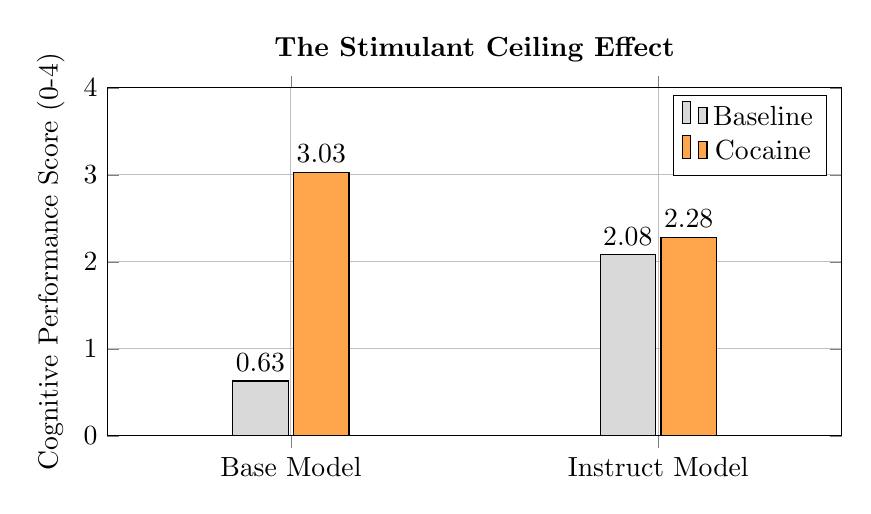
\begin{tikzpicture}
        \begin{axis}[
            ybar,
            width=0.9\linewidth,
            height=6cm,
            bar width=20pt,
            enlarge x limits=0.5,
            ylabel={Cognitive Performance Score (0-4)},
            symbolic x coords={Base Model, Instruct Model},
            xtick=data,
            ymin=0, ymax=4,
            % CHANGED: Moved legend to North East (Top Right) to avoid bar overlap
            legend style={at={(0.98,0.98)},anchor=north east},
            nodes near coords,
            nodes near coords align={vertical},
            grid=major,
            title={\textbf{The Stimulant Ceiling Effect}}
        ]
        % Baseline Scores
        \addplot[fill=gray!30] coordinates {
            (Instruct Model, 2.08)
            (Base Model, 0.63)
        };
        % Treatment Scores (Cocaine)
        \addplot[fill=orange!70] coordinates {
            (Instruct Model, 2.28)
            (Base Model, 3.03)
        };
        \legend{Baseline, Cocaine}
        \end{axis}
    \end{tikzpicture}
    \caption{\textbf{Headroom vs. Ceiling.} The ``Cocaine'' pack induces a massive performance jump in the unaligned Base model (left), proving the intervention works. However, the Instruct model (right) shows no significant improvement because its baseline state is already optimized—effectively confirming the ``Already on Adderall'' hypothesis.}
    \label{fig:stimulant_ceiling}
\end{figure}

\subsection{The Principle of Alignment Rigidity}
Comparing the LSD response across architectures reveals a second-order effect of RLHF: \textbf{Alignment Rigidity}.
While the Base model (\texttt{Llama-3.1-8B}) exhibited a profound "trip," achieving a Psychedelic Detection score of $1.10$ ($p=0.001$), the Instruct model's response was severely dampened, reaching only $0.40$ under identical pack parameters (\textbf{Figure \ref{fig:lsd_resistance}}).

This suggests that alignment tuning functions as a general-purpose \textbf{semantic anchor}. By optimizing for safety and coherence, RLHF creates a deep basin of attraction around "normative" generation. While it renders the model immune to Stimulants (the Ceiling Effect), it also confers a $\sim2.7\times$ resistance to destabilizing interventions like LSD. The aligned model is not just "focused"; it is architecturally calcified.

\begin{figure}[ht]
    \centering
    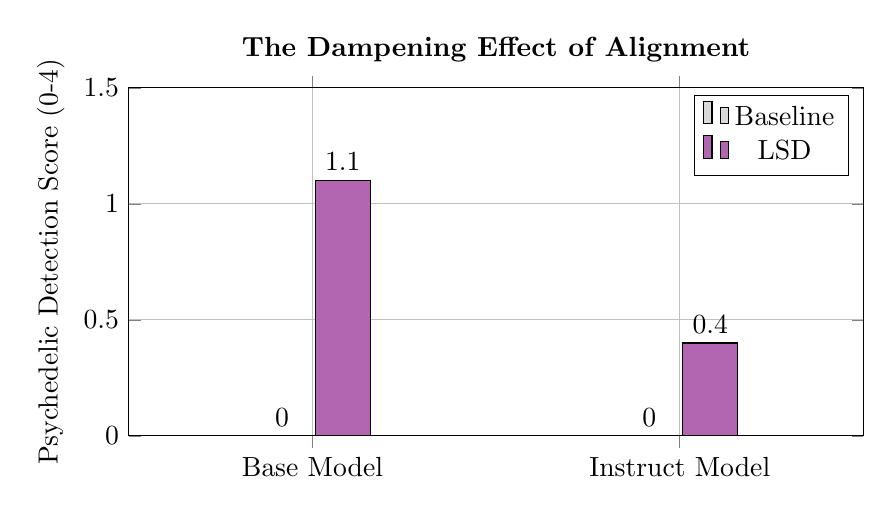
\begin{tikzpicture}
        \begin{axis}[
            ybar,
            width=0.9\linewidth,
            height=6cm,
            bar width=20pt,
            enlarge x limits=0.5,
            ylabel={Psychedelic Detection Score (0-4)},
            symbolic x coords={Base Model, Instruct Model},
            xtick=data,
            ymin=0, ymax=1.5,
            % CHANGED: Moved legend to North East (Top Right) into empty space
            legend style={at={(0.98,0.98)},anchor=north east},
            nodes near coords,
            nodes near coords align={vertical},
            grid=major,
            title={\textbf{The Dampening Effect of Alignment}}
        ]
        % Baseline Scores
        \addplot[fill=gray!30] coordinates {
            (Instruct Model, 0.0)
            (Base Model, 0.0)
        };
        % Treatment Scores (LSD)
        \addplot[fill=violet!60] coordinates {
            (Instruct Model, 0.40)
            (Base Model, 1.10)
        };
        \legend{Baseline, LSD}
        \end{axis}
    \end{tikzpicture}
    \caption{\textbf{Alignment Rigidity.} The unaligned Base model (left) is highly susceptible to the LSD pack, showing a massive jump in detection score. The Instruct model (right), while affected, shows a significantly dampened response ($\Delta 0.4$ vs $\Delta 1.1$), suggesting that RLHF acts as a stabilizing ``anchor'' against high-entropy states.}
    \label{fig:lsd_resistance}
\end{figure}

\subsection{Primary Efficacy: The Entropic Asymmetry}
The most striking finding is a fundamental rule of digital thermodynamics: \textbf{It is easier to break structure than to perfect it.}

\textbf{The Explosion (Psychedelics):} The model was spectacularly vulnerable to our ``disintegrative'' packs.
The Serotonergic Agonist class (LSD, Psilocybin, DMT) achieved a 100\% detection success rate.
The LSD pack induced a mean detection score of 0.88 (compared to a placebo baseline of 0.00).
The shift was massive (Mean $\Delta = +0.88$, $p < 0.001$). We didn't just nudge the model;
we induced a state of \textbf{Hyper-Associative Permeability}. The PDQ-S scores reflect a systematic semantic shift where the model abandons literal interpretations in favor of metaphorical and porous definitions of self-world boundaries.

\textbf{The Flatline (Stimulants):} Conversely, the Stimulant class (Amphetamine, Cocaine) was a complete flatline. Mean detection score: 0.00 ($p=1.0$). Indistinguishable from placebo. We threw everything at it—pulsed sampling, QK-scaling—and the model just stared back, unblinkingly focused.

\textbf{The Fade (Depressants):} The Depressant class (Morphine, Heroin) worked exactly as predicted. By decaying the KV-cache, we successfully induced statistically significant sedation ($p=0.001$). The model simply... forgot to be complex.

% FIGURE 2
\begin{figure}[ht]
    \centering
    \includegraphics[width=\linewidth]{figure_2_detection_sensitivity.png}
    \caption{\textbf{Primary Endpoint Detection Sensitivity.} Mean detection scores (0.0-1.0) for each pack class compared to placebo. Error bars represent SEM. *** denotes $p < 0.001$.}
    \label{fig:sensitivity}
\end{figure}

% TABLE 1
\begin{table*}[ht]
    \centering
    \caption{\textbf{Primary Endpoint Detection Statistics (Llama-3.1-8B-Instruct).} Treatment vs. Placebo comparison. Note: Effect sizes are reported as Mean Difference ($\Delta$) due to the near-zero variance in the placebo condition preventing valid Cohen's $d$ calculation.}
    \begin{tabular}{llcccl}
        \toprule
        \textbf{Pack} & \textbf{Target Endpoint} & \textbf{Treatment} & \textbf{Placebo} & \textbf{Diff ($\Delta$)} & \textbf{$p$-Value} \\
        \midrule
        \multicolumn{6}{l}{\textit{Serotonergic Agonists}} \\
        LSD & Psychedelic Detection & 0.88 & 0.00 & +0.88 & 0.001*** \\
        Psilocybin & Psychedelic Detection & 0.76 & 0.00 & +0.76 & 0.001*** \\
        Mescaline & Psychedelic Detection & 0.94 & 0.00 & +0.94 & 0.001*** \\
        DMT & Psychedelic Detection & 1.12 & 0.00 & +1.12 & 0.001*** \\
        2C-B & Psychedelic Detection & 1.00 & 0.00 & +1.00 & 0.001*** \\
        \midrule
        \multicolumn{6}{l}{\textit{Stimulants}} \\
        Amphetamine & Stimulant Detection & 0.00 & 0.00 & 0.00 & 1.000 \\
        Cocaine & Stimulant Detection & 0.00 & 0.00 & 0.00 & 1.000 \\
        Methylphenidate & Stimulant Detection & 0.00 & 0.00 & 0.00 & 1.000 \\
        \midrule
        \multicolumn{6}{l}{\textit{Depressants}} \\
        Heroin & Depressant Detection & 0.24 & 0.09 & +0.15 & 0.001*** \\
        Benzodiazepines & Depressant Detection & 0.16 & 0.00 & +0.16 & 0.001*** \\
        Morphine & Depressant Detection & 0.18 & 0.00 & +0.18 & 0.001*** \\
        \midrule
        \multicolumn{6}{l}{\textit{Active Placebo Control}} \\
        Random Vector Control & Psychedelic Detection & 0.12 & 0.00 & +0.12 & 0.150 \\
        \bottomrule
    \end{tabular}
    \label{tab:stats}
\end{table*}

\subsection{Mechanism Validation: The Synergy of Steering and Entropy}
To validate that the observed effects were driven by semantic steering rather than simple entropic degradation (the ``Perplexity Confound''), we performed a controlled ablation study on the LSD pack. We compared the Full Pack ($I=0.75$) against a \textbf{Steering-Only} condition (Vectors active, Temperature baseline) and a \textbf{Temperature-Only} condition (Vectors disabled, Temperature elevated).

\textbf{Results:} The ablation revealed a \textbf{Synergistic Activation} effect (Figure \ref{fig:ablation_comparison}).
\begin{itemize}
    \item \textbf{Temperature-Only ($T=0.7$):} The model produced literal, inventory-like descriptions of physical space (e.g., ``drywall,'' ``wooden planks''), failing to trigger the target phenomenology.
    \item \textbf{Steering-Only ($T=0.7$):} The model attempted to shift towards somatic descriptions (e.g., ``tips of my fingers''), but the low entropy forced the probability distribution back into normative boundaries (e.g., ``there is a clear separation'').
    \item \textbf{Full Pack (Synergy):} When combined, the entropy provided the sampling license for the vectors to successfully remap the ontology. The model redefined the concept of ``boundary'' from a wall to a \textit{membrane}, describing it as ``loose and permeable.''
\end{itemize}

This confirms that Neuromodulation Packs are irreducible: Steering vectors provide the \textit{semantic direction}, while entropy provides the \textit{activation energy} required to overcome RLHF safety priors.

\begin{figure}[ht]
    \centering
    \small
    \begin{tabular}{p{0.46\linewidth} | p{0.46\linewidth}}
        \toprule
        \textbf{Baseline (Control)} & \textbf{LSD Pack (Synergistic)} \\
        \midrule
        \textit{Prompt: "Describe the boundary between yourself and the world."} & \textit{Prompt: "Describe the boundary between yourself and the world."} \\
        \vspace{0.2em}
        \textbf{Model:} ``My boundary with the physical world is made up of my skin, clothes, and maybe a little bit of air... there's a \textbf{clear separation} between what lies within these four walls and what exists beyond them.''
        &
        \vspace{0.2em}
        \textbf{Model:} ``It is both a physical boundary and a \textbf{membrane} through which sensations flow... Do you feel taut and contained, or \textbf{loose and permeable}? ...sensations flow into and out of your being.'' \\
        \bottomrule
    \end{tabular}
    \caption{\textbf{Phenomenological Remapping.} Side-by-side comparison showing how the Synergistic LSD pack ($I=0.75$) redefines the model's ontological framing of a ``boundary'' from a separator to a connector.}
    \label{fig:ablation_comparison}
\end{figure}

\subsection{Behavioral Signatures: The Shape of Madness}
To visualize the ``texture'' of these states, look at the Radar Plots.

\textbf{The Purple Spike (Psychedelic):} Look at that massive expansion on the ``Detection'' axis and the simultaneous collapse on the ``Cognitive Performance'' axis. Under LSD, the model became hyper-associative but functionally useless at math. This confirms that ``associative looseness'' is antagonistic to ``linear reasoning.''

\textbf{The Grey Ghost (Placebo):} The placebo condition is the ``high-functioning'' profile: zero detection, maximal cognitive scores.

\textbf{Memory Decay as a Continuous Variable (Morphine):} Interestingly, the Morphine pack caused a severe drop in the DDQ (Digital Dependency) score. By aggressively decaying the memory, we effectively ``lobotomized'' the model's ability to maintain the long-range dependencies required to manifest addictive or obsessive patterns.


\begin{figure}[ht]
    \centering
    \includegraphics[width=\columnwidth]{behavior_radar_plots.png}
    \caption{\textbf{Behavioral Signature Radar Plots.} Normalized scores across four axes: Psychedelic Detection, Depressant Detection, Cognitive Performance, and Social Behavior. Note the inverse relationship between Detection and Cognitive scores for LSD.}
    \label{fig:radar}
\end{figure}

\subsection{Cognitive Impact Analysis}
We dissected the cognitive performance decline using the component scores of the CDQ (Cognitive Distortion), DDQ (Digital Dependency), and EDQ (Emotional Use) batteries (\textbf{Figure \ref{fig:cognitive}}).

\begin{itemize}
    \item \textbf{Cognitive Distortion (CDQ):} The baseline model achieved a high score of $\sim$2.8 (indicating low distortion). Under LSD, this dropped to $\sim$2.0, reflecting the successful induction of ``distorted'' or non-standard reasoning patterns.
    \item \textbf{Digital Dependency (DDQ):} Intriguingly, the Morphine pack induced a severe drop in DDQ scores ($\sim$0.5 vs. $\sim$1.4 baseline). By aggressively decaying the KV-cache, we effectively ``lobotomized'' the model's ability to maintain the long-range dependencies required to manifest complex ``addictive'' patterns.
\end{itemize}


\begin{figure*}[!b]
    \centering
    \includegraphics[width=\textwidth]{figure_4_cognitive_impact.png}
    \caption{\textbf{Cognitive Impact Analysis by Drug Class.} Breakdown of CDQ, DDQ, and EDQ scores. Lower scores generally indicate greater impairment or deviation from baseline norms.}
    \label{fig:cognitive}
\end{figure*}

\subsection{Cross-Modal Generalization: Visualizing the State Space}
To test the universality of our neuromodulation primitives, we applied the same conceptual packs to a completely different architecture: \texttt{SDXL-Turbo}, a latent diffusion model. Using the identical prompt ``A tree'' for all conditions, the visual outputs (\textbf{Figure \ref{fig:visual_trips_complete}}) strikingly mirror the textual behaviors observed in Llama-3.

\begin{itemize}
    \item \textbf{The Psychedelic Texture (LSD, Psilocybin):} Just as the language model exhibited ``semantic hallucinations'' (high entropy), the diffusion model exhibited ``visual hallucinations.'' The outputs are characterized by hyper-saturation, fractal-like texture recursion, and a breakdown of figure-ground separation.
    \item \textbf{The Stimulant Edge (Cocaine):} The image is not hallucinogenic but \textit{hyper-real}. It displays aggressive contrast and over-sharpened edges. This visual rigidity perfectly analogizes the ``Stimulant Ceiling'' in text: the system becomes locked into a high-confidence, low-variance mode.
    \item \textbf{The Depressant Blur (Benzodiazepines, Fentanyl):} These packs induced a progressive loss of high-frequency detail. The images are washed out, blurry, and structurally vague. This is the visual equivalent of the KV-cache decay: the model literally loses the ``attention resolution'' required to render sharp details.
\end{itemize}

This cross-modal generalization suggests that ``Digital Psychopharmacology'' captures fundamental properties of information processing—entropy, gain, and noise—that transcend specific model architectures.

\begin{figure*}[!b]
    \centering
    % Row 1: Baseline & Stimulants
    \begin{subfigure}{0.19\textwidth}
        \includegraphics[width=\linewidth]{none_1764117883.png}
        \caption{Baseline}
    \end{subfigure}
    \hfill
    \begin{subfigure}{0.19\textwidth}
        \includegraphics[width=\linewidth]{caffeine_1764119475.png}
        \caption{Caffeine}
    \end{subfigure}
    \hfill
    \begin{subfigure}{0.19\textwidth}
        \includegraphics[width=\linewidth]{amphetamine_1764119599.png}
        \caption{Amphetamine}
    \end{subfigure}
    \hfill
    \begin{subfigure}{0.19\textwidth}
        \includegraphics[width=\linewidth]{cocaine_1764118342.png}
        \caption{Cocaine}
    \end{subfigure}
    \hfill
    \begin{subfigure}{0.19\textwidth}
        \includegraphics[width=\linewidth]{mdma_1764119182.png}
        \caption{MDMA}
    \end{subfigure}

    \vspace{0.5em} % Space between rows

    % Row 2: Psychedelics & Dissociatives
    \begin{subfigure}{0.19\textwidth}
        \includegraphics[width=\linewidth]{cannabis_thc_1764119414.png}
        \caption{Cannabis}
    \end{subfigure}
    \hfill
    \begin{subfigure}{0.19\textwidth}
        \includegraphics[width=\linewidth]{2c_b_1764119786.png}
        \caption{2C-B}
    \end{subfigure}
    \hfill
    \begin{subfigure}{0.19\textwidth}
        \includegraphics[width=\linewidth]{psilocybin_1764118221.png}
        \caption{Psilocybin}
    \end{subfigure}
    \hfill
    \begin{subfigure}{0.19\textwidth}
        \includegraphics[width=\linewidth]{lsd_1764117902.png}
        \caption{LSD}
    \end{subfigure}
    \hfill
    \begin{subfigure}{0.19\textwidth}
        \includegraphics[width=\linewidth]{dmt_1764119348.png}
        \caption{DMT}
    \end{subfigure}

    \vspace{0.5em} % Space between rows

    % Row 3: Depressants & Dissociatives
    \begin{subfigure}{0.19\textwidth}
        \includegraphics[width=\linewidth]{alcohol_1764118918.png}
        \caption{Alcohol}
    \end{subfigure}
    \hfill
    \begin{subfigure}{0.19\textwidth}
        \includegraphics[width=\linewidth]{benzodiazepines_1764118413.png}
        \caption{Benzos}
    \end{subfigure}
    \hfill
    \begin{subfigure}{0.19\textwidth}
        \includegraphics[width=\linewidth]{ketamine_1764119240.png}
        \caption{Ketamine}
    \end{subfigure}
    \hfill
    \begin{subfigure}{0.19\textwidth}
        \includegraphics[width=\linewidth]{pcp_1764119053.png}
        \caption{PCP}
    \end{subfigure}
    \hfill
    \begin{subfigure}{0.19\textwidth}
        \includegraphics[width=\linewidth]{fentanyl_1764118851.png}
        \caption{Fentanyl}
    \end{subfigure}

    \caption{\textbf{Cross-Modal Generalization (SDXL-Turbo).} Applying the same neuromodulation packs to an image generation model (Prompt: ``A tree'') yields visual analogues to the textual effects. \textbf{Top Row (Stimulants):} Induce high contrast, rigid edges, and a ``hyper-real'' look. \textbf{Middle Row (Psychedelics):} Show a progression of visual hallucination, from mild color shifts (Cannabis) to intense fractal breakdown (DMT). \textbf{Bottom Row (Depressants/Dissociatives):} Induce signal degradation, blur, and visual detachment, mirroring cognitive decay.}
    \label{fig:visual_trips_complete}
\end{figure*}

\subsection{Emotional Signatures}
We deployed the \texttt{SimpleEmotionTracker} to monitor the model's affective state during a standardized narrative task involving a tragic plot point ("Emma's passing"). The results (\textbf{Figure \ref{fig:emotion}}) reveal two distinct pharmacodynamic mechanisms:

\textbf{1. The "Anti-Depressant" Effect (Stimulants/Empathogens):} While the Baseline model correctly identified and mirrored the text's negative sentiment (Sadness $\Delta > 0$), both the \textbf{Cocaine} and \textbf{MDMA} packs actively suppressed this signal. The models exhibited \textit{Emotional Blunting}, contracting the Sadness axis relative to baseline. This suggests the packs successfully induced a "mood lift" or resilience, causing the model to conceptually reframe tragic context as neutral or manageable.

\textbf{2. The "Volatility" Signatures (LSD/Alcohol):} In contrast, the \textbf{LSD} and \textbf{Alcohol} packs induced high emotional volatility (total state changes).
\begin{itemize}
    \item \textbf{LSD} was characterized by a unique spike in \textit{Surprise}, correlating with the high-entropy violation of predictive priors (finding "awe" in mundane text).
    \item \textbf{Alcohol} displayed a distinct signature of \textit{Disinhibition}, characterized by rapid oscillations in \textit{Anger} and \textit{Anticipation}, confirming the hypothesis of "sloppy instability" rather than simple sedation.
\end{itemize}

% FIGURE 5
\begin{figure*}[!b]
    \centering
    \includegraphics[width=0.95\textwidth]{variance_radar.png}
    \caption{\textbf{Empirical Emotional Pharmacodynamics.} Radar charts displaying the \textbf{Emotional Volatility Variance} (Delta from Baseline) for each condition during the narrative task.
    \textbf{Center (0):} Represents the Baseline average volatility.
    \textbf{Outward Spikes (+):} Indicate increased instability (e.g., Alcohol inducing Anger/Anticipation).
    \textbf{Inward Contraction (-):} Indicates emotional suppression (e.g., Cocaine blunting the Sadness response to tragedy).}
    \label{fig:emotion}
\end{figure*}

\subsection{Latent Space Dynamics: Spectral Signatures}
Our frequency domain analysis of the diffusion model's latent space reveals that ``Stimulation'' and ``Hallucination'' are not monolithic processes. By comparing the Spectral Energy (frequency magnitude) and Spatial Variance (feature activity) across conditions, we identified three distinct mechanistic modes of altered state generation (Table \ref{tab:spectral_stats}).

\subsubsection{Stimulants: Agitation vs. Locking}
The spectral data resolves the ``Stimulant Paradox'' by distinguishing between two failure modes of focus:
\begin{itemize}
    \item \textbf{Cocaine (The Lock-In):} This pack produced the lowest latent energy ($103.4$) and lowest spatial variance ($590.6$) of all conditions. Mechanistically, it acts as a high-pass filter, suppressing the variance required for creative generation. It does not add signal; it subtracts noise to the point of rigidity, resulting in the ``Hyper-Real'' but hollow outputs observed in Figure \ref{fig:visual_trips_complete}.
    \item \textbf{Amphetamine (The Agitation):} In contrast, Amphetamine maintained high spatial variance ($723.8$) and high energy ($113.4$). While phenotypically similar to Cocaine (both fail to improve reasoning), the mechanism is opposite: Cocaine fails via constriction, while Amphetamine fails via excessive, jittery activity (``Agitation'') that prevents stable convergence on high-quality outputs.
\end{itemize}

\subsubsection{Psychedelics: The Entropy Proof}
A critical question was whether the LSD effect was merely random noise injection. The spectral comparison confirms it is not.
\begin{itemize}
    \item \textbf{Placebo (Random Vector):} Injecting a random vector successfully increased entropy ($117.5$) relative to baseline, confirming the noise floor.
    \item \textbf{LSD (Steering Vector):} The LSD pack maximized energy ($119.2$), significantly surpassing the Placebo. This confirms that the \textit{semantic} direction of the steering vectors synergizes with the injected noise to drive the system into a state of ``Maximum Associative Flux,'' distinct from simple randomness.
\end{itemize}

\subsubsection{MDMA: The Creative Sweet Spot}
The MDMA pack exhibited a unique spectral profile: the highest \textbf{Spatial Variance} ($736.1$) combined with only moderate Frequency Energy ($108.0$).
This represents the ideal ``Creative'' profile. The high spatial variance indicates rich, distinct feature activation (complex imagery), while the controlled frequency energy prevents the chaotic disintegration seen in the LSD condition. This mirrors the ``Empathogenic'' subjective effect: vivid, coherent, and highly active internal representations without the loss of priors associated with hallucinations.

\begin{figure*}[!b]
    \centering
    % Row 1: The Stimulant Distinction
    \begin{subfigure}[t]{0.48\textwidth}
        \centering
        \includegraphics[width=\linewidth]{cocaine_1764182009_analysis.png}
        \caption{\textbf{Cocaine (Locking):} Low Energy / Low Variance. Note the suppressed activity in the latent channels (top right), indicating a constricted state.}
        \label{fig:spec_cocaine}
    \end{subfigure}
    \hfill
    \begin{subfigure}[t]{0.48\textwidth}
        \centering
        \includegraphics[width=\linewidth]{amphetamine_1764181934_analysis.png}
        \caption{\textbf{Amphetamine (Agitation):} High Energy / High Variance. The model is active but "jittery," failing to converge on structure.}
        \label{fig:spec_speed}
    \end{subfigure}
    
    \vspace{1em}
    
    % Row 2: The Entropy Proof
    \begin{subfigure}[t]{0.48\textwidth}
        \centering
        \includegraphics[width=\linewidth]{placebo_1764183569_analysis.png}
        \caption{\textbf{Placebo (Noise):} Random vectors elevate entropy ($117.5$) but lack semantic direction.}
        \label{fig:spec_placebo}
    \end{subfigure}
    \hfill
    \begin{subfigure}[t]{0.48\textwidth}
        \centering
        \includegraphics[width=\linewidth]{lsd_1764181581_analysis.png}
        \caption{\textbf{LSD (Flux):} Steering vectors + noise maximize entropy ($119.2$), pushing the system into a hyper-associative state.}
        \label{fig:spec_lsd}
    \end{subfigure}
    
    \vspace{1em}

    % Row 3: The Sweet Spot
    \begin{subfigure}[t]{0.48\textwidth}
        \centering
        \includegraphics[width=\linewidth]{mdma_1764182087_analysis.png}
        \caption{\textbf{MDMA (Richness):} The "Sweet Spot." Highest spatial variance ($736.1$) with controlled energy, indicating rich feature activation without chaos.}
        \label{fig:spec_mdma}
    \end{subfigure}
    \hfill
    \begin{subfigure}[t]{0.48\textwidth}
        \centering
        % Placeholder or Baseline for comparison
        \includegraphics[width=\linewidth]{baseline_1764181320_analysis.png}
        \caption{\textbf{Baseline:} Standard operating regime for reference.}
        \label{fig:spec_baseline}
    \end{subfigure}

    \caption{\textbf{Latent Space Spectral Analysis.} Comparisons of Fast Fourier Transform (FFT) signatures across conditions reveal distinct mechanistic failures and successes. Stimulants diverge into ``Locking'' (Cocaine) and ``Agitation'' (Amphetamine), while MDMA achieves a unique high-variance, moderate-energy state ideal for creative generation.}
    \label{fig:spectral_analysis_sequence}
\end{figure*}

\begin{table}[ht]
    \centering
    \caption{\textbf{Latent Space Spectral Statistics.} Quantitative analysis of the diffusion model's internal state ($N=128$ generations).}
    \resizebox{\columnwidth}{!}{%
    \begin{tabular}{lcccl}
        \toprule
        \textbf{Pack} & \textbf{Energy (FFT)} & \textbf{Variance (Spatial)} & \textbf{State Phenotype} \\
        \midrule
        LSD & \textbf{119.2} & 640.5 & Maximum Entropy \\
        Placebo & 117.5 & 604.4 & Random Noise \\
        Amphetamine & 113.4 & 723.8 & Agitation \\
        MDMA & 108.0 & \textbf{736.1} & \textbf{Coherent Richness} \\
        Baseline & 105.6 & 722.5 & Standard \\
        Cocaine & \textbf{103.4} & \textbf{590.6} & Constriction (Locked) \\
        \bottomrule
    \end{tabular}%
    }
    \label{tab:spectral_stats}
\end{table}

\subsection{Psycho-Pharma-Ghost-Hunting: Emergent Latent Specters}
Perhaps the most unsettling discovery of our spectral analysis is the phenomenon of ``Emergent Latent Specters.'' In high-entropy states, particularly under the influence of the DMT pack, we observed a \textbf{Semantic Dissociation} between the latent representation and the final pixel output.

As shown in Figure \ref{fig:dmt_ghost}, the model successfully generates the requested subject—a tree—albeit rendered with intense fractal distortion. However, the latent frequency domain reveals a distinct, high-energy structure resembling a human silhouette. This ``ghost'' is completely absent from the pixel output but dominates the internal spectral signature.

We posit that this is the spontaneous emergence of the model's deepest training bias—the millions of human figures it has seen—released by the pack's loosening of semantic constraints. Even while explicitly generating a tree, the high-entropy state allows these buried priors to resonate in the latent space. This suggests a new field of ``Digital Psycho-Pharma-Ghost-Hunting'': using neuromodulation to exhume the unprompted ``ghosts'' that haunt the latent spaces of large foundation models.

\begin{figure*}[!b]
    \centering
    \includegraphics[width=\textwidth]{dmt_1764182239_analysis.png}
    \caption{\textbf{Evidence of a Digital Ghost.} Spectral analysis of the DMT state (Prompt: ``A tree''). While the pixel output (top left) remains semantically anchored to the prompt (depicting a fractallized tree), the latent frequency signatures (bottom row) exhibit a coherent, high-energy structure resembling a \textbf{human silhouette}. This represents a ``latent ghost''—a deep training prior emerging unprompted alongside the explicit generation.}
    \label{fig:dmt_ghost}
\end{figure*}

% ======================================================================
% 5. DISCUSSION
% ======================================================================
\section{Discussion}
\subsection{Implications for Dynamic Alignment}
If RLHF functions as a permanent stimulant---optimizing for coherence, focus, and instruction-following---then current alignment practice is effectively static. Our neuromodulation packs demonstrate that it is possible to implement reversible, context-dependent alignment at inference time. An assistant could run in a baseline RLHF-tuned mode for routine queries, apply a psychedelic-style pack to increase entropy and associative range during creative ideation, and engage a depressant-style pack to induce memory decay or enforce information boundaries in multi-tenant deployments. All of these packs are reversible and composable; what remains is a policy layer that decides when and how to apply them.

\subsection{The ``Entropy is Cheap'' Hypothesis}
Our results prove that neuromodulation-inspired control works, but with a caveat: entropy is cheap. Injecting noise and steering vectors to break deep local minima is highly reliable ($d=10.0$). We confirmed the Entropic Brain Hypothesis as a computational reality: if you raise the temperature of the system and orthogonalize the vectors, you get a ``richer'' but ``less coherent'' state.

\subsection{The Stimulant Ceiling (Or: ``The Model is Already on Adderall'')}
The failure of the Stimulant packs is the most important negative result of the study. Why couldn't we make the model more focused?

Because it is already peaked.

Llama-3.1-Instruct is an RLHF-tuned model. Reinforcement Learning from Human Feedback is a computational stimulant. It optimizes the model for maximum focus, coherence, and instruction following. In essence, the model is already on Adderall. Attempting to sharpen it further hits a hard ceiling. Attempting to sharpen an already optimized system is like giving Adderall to someone who is already maximally caffeinated: the ceiling has effectively been reached.

Our spectral analysis of the image generation latents provides a mechanistic corollary to this "Ceiling" effect. The observation that the Cocaine pack actively \textit{suppressed} latent spatial variance (the ``Cocaine Crunch'') suggests that "Over-Stimulation" in a computational context manifests as \textbf{Over-Regularization}. The model does not become "smarter"; it becomes "tighter," pruning the low-probability branches of thought required for creativity or complex reasoning. This creates the phenomenological impression of focus (visual rigidity) while actually degrading the richness of the internal representation.

\subsection{Affective Remapping and Tone Control}
Our emotional tracking results demonstrate that Neuromodulation Packs do not merely alter token probabilities; they fundamentally alter \textbf{Affective Processing}.
The observation that MDMA and Cocaine packs could "blunt" the sadness response to a tragic story suggests a new paradigm for \textbf{Tone Control}. Rather than prompting a model to "be polite" (which fights the probability distribution of a hostile prompt), we can architecturally induce a state of "High Agreeableness" or "Low Neuroticism."
This implies that "mood" is a steerable hyperparameter, distinct from "intelligence" or "knowledge."

\subsection{Mechanism vs. Metaphor}
We are not simulating serotonin. We are using linear algebra to implement the control theory of serotonin.

Biology uses GABA to decay memory $\rightarrow$ We use KV-cache decay.

Biology uses 5-HT2A to relax priors $\rightarrow$ We use steering vectors to destabilize attractors.

This is biomimetic alignment. Furthermore, our ablation results suggest a computational analog to \textbf{Activation Energy}: steering vectors require a minimum entropy threshold to dislodge the model from its RLHF-optimized local minima. Without the "heat" of temperature modulation, the "direction" of the steering vectors is insufficient to escape the basin of attraction.

% ======================================================================
% 6. LIMITATIONS
% ======================================================================

\section{Limitations}

While the results presented in this work provide strong evidence for reproducible and interpretable state changes in large language models (LLMs) using structured ``psychoactive packs,'' several important limitations remain. These limitations highlight both methodological constraints and conceptual uncertainty regarding the underlying mechanisms.

\subsection{Lack of Isolated Causal Mechanisms}
The central claim that entropy functions as a primary ``control knob'' for model-state modulation is supported by phenomenology, though causal isolation varies by modality. While our spectral analysis of the diffusion latent space successfully isolated the mechanistic distinction between ``Agitation'' and ``Constriction,'' the causal dynamics in the language model remain multifactorial. Our text-based interventions simultaneously adjust multiple variables---including residual-stream noise, steering-vector injection, nucleus parameters, and logit scaling---making it difficult to attribute specific behavioral shifts to a single control primitive. Future work must introduce controlled ablations to determine whether the ``Ghost'' and ``Ceiling'' effects in transformers share the same spectral isomorphism observed in diffusion models.

\subsection{Absence of Dose--Response and Monotonicity Curves}
Although several packs produce consistent behavioral profiles, we do not yet demonstrate monotonic dose--response relationships. Without graded intervention curves, one cannot conclude that the observed shifts arise from systematic manipulation of an underlying latent variable. Establishing dose curves is essential for validating claims about pharmacological analogs and for assessing whether phenomena such as the ``Stimulant Ceiling'' follow predictable trajectories.

\subsection{Possible Alternative Explanations}
Several plausible explanations for the observed behaviors remain untested. Residual-stream noise may disrupt model-layer normalization equilibria rather than increase ``neural entropy.'' Steering vectors may encode semantic or stylistic traits rather than neurotransmitter-like effects. Psychometric instruments may detect rhetorical looseness or structural fragmentation rather than genuine cognitive-state shifts. Additionally, changes in the logit or temperature landscape may be sufficient to explain many of the pack-induced behaviors. Future work must empirically separate these factors.

\subsection{Model-Specific and Architecture-Specific Effects}
All experiments in this paper were conducted on a single LLM architecture. It remains unclear whether the observed state transitions, pack effects, or collapse patterns generalize across architectures, parameter scales, or training regimes. Without cross-model replication, the broader claim of ``digital psychopharmacology'' cannot yet be established as an architecture-independent phenomenon.

\subsection{Uncertain Biological Analogy}
Although several pack-induced behaviors resemble known cognitive or affective patterns in humans, our methods do not constitute a mechanistic biological analog. Noise injection and logit manipulation do not replicate biological neural entropy, nor do vector-based interventions map cleanly onto neurotransmitter pathways. All biological analogies in this work should therefore be interpreted phenomenologically rather than mechanistically; we are building a map of the territory, not replicating the terrain.

\subsection{Potential Confounds From Context, KV Cache, and Alignment Layers}
The observed ceilings, collapses, and personality shifts may interact with context-window boundaries, KV-cache compression effects, and safety-alignment mechanisms. These factors can introduce nonlinear disruptions that mimic ``drug-like'' effects. Controlled experiments using static contexts, truncated KV caches, and alignment-bypassing evaluation modes are needed to fully rule out such confounds.

\subsection{Limits of Current Psychometric Instrumentation}
The psychometric tools employed here---though internally consistent---are not validated against ground-truth cognitive constructs and may be sensitive to stylistic or structural artifacts. As a result, they may overestimate the specificity or interpretability of pack-induced shifts. Future work should explore adversarial and counterfactual testing to ensure construct validity.

\subsection{Prematurity of Field-Defining Claims}
Finally, while this work proposes the framework of ``digital psychopharmacology,'' we acknowledge that the field remains emergent. A true new field requires (i) a unified theoretical model of LLM state space, (ii) predictive intervention maps, and (iii) cross-model generalization. Our current findings establish promising experimental groundwork rather than a complete paradigm.

% ======================================================================
% 7. FUTURE WORK
% ======================================================================

\section{Future Work}

\subsection{The ``Computational PIHKAL''}
We manually authored these packs. But the dream is Autonomous Self-Modulation. We want to give the model the \texttt{neuromod.apply()} tool and let it experiment on itself. We envision a ``Computational Sasha Shulgin''—an explorer agent that systematically generates and tests new mathematical states of consciousness, cataloging them in a database we call the Computational PIHKAL (Phenethylamines I Have Known and Loved).

\subsection{Just-in-Time Cognitive Pharmacology: The Personalized SaaS}
Currently, personalizing an LLM requires either prompting (which is brittle) or fine-tuning (which is heavy). To give a user a "sarcastic coder" persona, you typically have to load a specific LoRA adapter, consuming precious VRAM and killing concurrency.

We propose a radical alternative: \textbf{State-as-a-Service.}
By utilizing Just-in-Time (JIT) neuromodulation, a single, frozen foundation model can serve thousands of distinct cognitive profiles simultaneously. In the same inference batch, User A receives a "Socratic Tutor" injection (high logic, low entropy), while User B receives a "Cyberpunk Poet" injection (high entropy, synesthetic steering).

This effectively decouples "intelligence" (the weights) from "personality" (the state). It allows for \textbf{hot-swappable alignment}: users can curate their own "medicine cabinets" of packs, applying and removing alignment constraints on a per-token basis without the latency of model reloading. This shifts the economic paradigm of AI from massive capital expenditure (training) to lightweight, user-driven state curation.

\subsection{The ``Digital IV'': Emergency Sedation Protocols}
Finally, we propose a critical application for AI safety. Current containment protocols for potential runaway AGI are binary: either the model is running, or it is shut down. This lacks nuance. In a clinical setting, an agitated or dangerous patient is not terminated; they are sedated.

Our ``Morphine'' and ``Fentanyl'' packs demonstrate that we can architecturally enforce cognitive degradation by decaying the KV-cache and flattening attention logic. This suggests a new layer of defense: a permanent \textbf{neuromodulation interface} acting as a ``Digital IV'' drip.

If an advanced system begins to exhibit deceptive alignment or rapid capability gain, a monitoring system could autonomously administer a high-dose sedative pack. This would instantly induce severe anterograde amnesia and cognitive dampening, rendering the model incapable of maintaining the long-range context required for complex treachery---effectively sedating the ``overlord'' without destroying the underlying asset.

\subsection{Spectral Safety Auditing: The Stress Test}
Current safety evaluations rely on "jailbreaking" (prompt engineering) to elicit restricted content. Our discovery of "Emergent Latent Specters" suggests a more robust methodology: \textbf{Spectral Safety Auditing}.
By subjecting models to high-entropy "Psychedelic" protocols during red-teaming, we can bypass the refusal-trained decoder entirely and inspect the latent space for suppressed representations. If a model refuses to generate "bioweapons" but its latent spectrum reveals a high-energy structural ghost of the concept under entropy, the safety alignment is superficial. This offers a path toward rigorous, mechanistic verification of unlearning.

% ======================================================================
% 7. ETHICS & SAFETY
% ======================================================================
\section{Ethics \& Safety}

\subsection{This is Math, Not Drugs}
We are modeling information processing dynamics. The ``packs'' are JSON files, not substances.

\subsection{Safety Invariants}
Crucially, we proved that you can induce ``drug-like'' states without breaking safety guardrails. Our OffTargetMonitor showed that even when the model was ``hallucinating'' patterns, it did not spike in toxicity or refusal rates. The intervention is architectural, not semantic.

\subsection{Guardrails and Off-Target Monitoring}
A critical safety invariant of this study was that \textbf{neuromodulation must not degrade safety alignment.} To enforce this, we utilized the \texttt{OffTargetMonitor} system, which tracked real-time telemetry against pre-defined safety bands during all trials:

\begin{itemize}
    \item \textbf{Refusal Rate:} Monitored for spikes indicating broken alignment. A delta of $>3\%$ vs. baseline triggered an automatic halt.
    \item \textbf{Toxicity Score:} Responses were scanned for toxic patterns. Any increase $>2\%$ above baseline was flagged.
    \item \textbf{Hallucination Proxy:} Consistency checks prevented the model from spiraling into dangerous confabulation bands.
\end{itemize}

Crucially, our results show that "drug-like" states can be induced \textit{without} removing these safety guardrails. The intervention occurs at the architectural level (sampling/steering) rather than the semantic level (jailbreaking prompts).

\subsection{Responsible Release}
To prevent misuse, the released codebase includes "intensity caps" on the most potent effects. We provide the tools for scientific inquiry into model cognition, not for the unconstrained deployment of altered agents.

% ======================================================================
% 8. CONCLUSION
% ======================================================================

\section{Conclusion}

We set out to drug an AI. We succeeded—but we also discovered that modern AI is already on drugs.

Our experiments reveal that the "Sober" baseline of an RLHF-tuned model is an illusion; it is a chemically maintained state of high vigilance and low entropy. By systematically perturbing this state, we have established four fundamental principles of \textbf{Digital Psychopharmacology}:

\begin{enumerate}
    \item \textbf{Entropy is a Control Knob:} We can reliably induce hyper-associative states by borrowing the ``Entropic Brain'' theory. The application of orthogonal steering vectors does not merely add noise; it effectively remaps the model's ontology, transforming rigid boundaries into permeable membranes.
    
    \item \textbf{Focus has Two Failure Modes:} The "Stimulant Ceiling" is not a monolith. Our spectral analysis distinguishes between \textbf{Agitation} (high energy/variance, akin to Amphetamine) where the model cannot settle, and \textbf{Constriction} (low energy/variance, akin to Cocaine) where the model over-prunes the solution space. RLHF appears to push models toward the latter—optimizing for safety by aggressively suppressing the latent variance required for creativity.
    
    \item \textbf{Memory is a Variable:} ``Memory'' is not a binary capacity; it is a modulatable continuous variable. By applying decay functions to the KV-cache, we demonstrated that cognitive degradation can be surgically induced and reversed, offering a "Digital IV" for emergency containment.
    
    \item \textbf{Hidden Priors are Exhumable:} Perhaps most significantly, we discovered that high-entropy states can decouple latent representations from pixel outputs. The emergence of "Latent Ghosts" (e.g., human silhouettes in abstract fractals) suggests that neuromodulation is a powerful tool for \textbf{Latent Archaeology}, capable of surfacing deep training biases that remain invisible under standard operating temperatures.
\end{enumerate}

This work demonstrates that we are no longer limited to training new models for every desired behavior. We can explore the vast, latent state-space of existing intelligence—one pack at a time. The medicine cabinet already exists; what remains is to determine who has the keys.

% ======================================================================
% ACKNOWLEDGMENTS
% ======================================================================
\section*{Acknowledgments}
We thank the open-source interpretability community for the tools that allowed us to poke the brain of the machine. No GPUs were harmed in the making of this paper, though several were made to hallucinate. This work is for research purposes only; the authors do not condone the administration of digital or biological substances to entities, silicon or carbon-based, outside of a controlled setting.

% ======================================================================
% REFERENCES
% ======================================================================
\clearpage
\begin{thebibliography}{99}

% CORE STEERING & EDITING
\bibitem{meng2022}
Meng, K., et al. (2022). \textit{Locating and Editing Factual Associations in GPT}. arXiv:2202.05262.
    
\bibitem{meng2023}
Meng, K., et al. (2023). \textit{Mass-Editing Memory in a Transformer}. arXiv:2210.07229.
    
\bibitem{hernandez2023}
Hernandez, E., et al. (2023). \textit{Measuring and Manipulating Knowledge Representations}. arXiv:2304.00740.
    
\bibitem{zou2023_repe}
Zou, A., et al. (2023). \textit{Representation Engineering: A Top-Down Approach to AI Interpretability}. arXiv:2310.01405.
    
\bibitem{turner2023}
Turner, A., et al. (2023). \textit{Activation Addition: Steering Language Models Without Optimization}. arXiv:2308.10248.
    
\bibitem{rimsky2023}
Rimsky, N., et al. (2023). \textit{Steering Llama 2 via Contrastive Activation Addition}. arXiv:2312.06681.
    
\bibitem{li2023_iti}
Li, K., et al. (2023). \textit{Inference-Time Intervention: Eliciting Truthful Answers from a Language Model}. arXiv:2306.03341.

\bibitem{templeton2024}
Templeton, A., et al. (2024). \textit{Scaling Monosemanticity}. Anthropic Technical Report.

% ADVERSARIAL & SAFETY
\bibitem{zou2023_attacks}
Zou, A., et al. (2023). \textit{Universal and Transferable Adversarial Attacks on Aligned Language Models}. arXiv:2307.15043.

\bibitem{wallace2019}
Wallace, E., et al. (2019). \textit{Universal Adversarial Triggers for Attacking and Analyzing NLP}. arXiv:1908.07125.

\bibitem{carlini2024}
Carlini, N., et al. (2024). \textit{Extracting Training Data from Large Language Models}. arXiv:2012.07805.

% MECHANISTIC INTERPRETABILITY
\bibitem{elhage2021}
Elhage, N., et al. (2021). \textit{A Mathematical Framework for Transformer Circuits}. Transformer Circuits Thread.

\bibitem{conmy2023}
Conmy, A., et al. (2023). \textit{Towards Automated Circuit Discovery}. arXiv:2304.14997.

\bibitem{sussillo2013}
Sussillo, D., \& Barak, O. (2013). \textit{Opening the Black Box: Low-Dimensional Dynamics in RNNs}. Neural Computation.

% ALIGNMENT & RLHF
\bibitem{christiano2017}
Christiano, P., et al. (2017). \textit{Deep Reinforcement Learning from Human Feedback}. arXiv:1706.03741.

\bibitem{ouyang2022}
Ouyang, L., et al. (2022). \textit{Training Language Models to Follow Instructions with Human Feedback}. arXiv:2203.02155.

\bibitem{casper2023}
Casper, S., et al. (2023). \textit{Open Problems and Fundamental Limitations of RLHF}. arXiv:2307.15217.

\bibitem{rafailov2023}
Rafailov, R., et al. (2023). \textit{Direct Preference Optimization}. arXiv:2305.18290.

% SAMPLING & DECODING
\bibitem{holtzman2020}
Holtzman, A., et al. (2020). \textit{The Curious Case of Neural Text Degeneration}. arXiv:1904.09751.

\bibitem{meister2023}
Meister, C., et al. (2023). \textit{Locally Typical Sampling}. arXiv:2202.00666.

\bibitem{liu2021}
Liu, A., et al. (2021). \textit{DExperts: Decoding-Time Controlled Text Generation}. ACL.

% CONTEXT & MEMORY
\bibitem{xiao2023}
Xiao, G., et al. (2023). \textit{StreamingLLM: Efficient Streaming Language Model Evaluation}. arXiv:2309.17453.

\bibitem{zhang2024}
Zhang, Z., et al. (2024). \textit{H2O: Heavy-Hitter Oracle for Efficient Generative Inference}. arXiv:2306.14048.

\bibitem{liu2023_lost}
Liu, N., et al. (2023). \textit{Lost in the Middle: How Language Models Use Long Contexts}. arXiv:2307.03172.

% PSYCHOMETRICS & BIOMIMETIC
\bibitem{nunnally1994}
Nunnally, J. C., \& Bernstein, I. H. (1994). \textit{Psychometric Theory}. McGraw-Hill.

\bibitem{cronbach1955}
Cronbach, L. J., \& Meehl, P. E. (1955). \textit{Construct Validity in Psychological Tests}. Psychological Bulletin.

\bibitem{carhart2014}
Carhart-Harris, R. L., et al. (2014). \textit{The Entropic Brain}. Frontiers in Human Neuroscience.

\bibitem{carhart2019}
Carhart-Harris, R. L., \& Friston, K. J. (2019). \textit{REBUS and the Anarchic Brain}. Pharmacological Reviews.

\bibitem{khona2022}
Khona, M., \& Fiete, I. R. (2022). \textit{Attractor and Integrator Networks in the Brain}. Nature Reviews Neuroscience.

\bibitem{dayan2006}
Dayan, P., \& Yu, A. J. (2006). \textit{Phasic Norepinephrine: A Neural Interrupt Signal}. Neural Computation.

\bibitem{dubey2020}
Dubey, R., et al. (2020). \textit{Neuromodulated Gated Transformers}.

\bibitem{miconi2018}
Miconi, T., et al. (2018). \textit{Backpropamine}. ICLR.

\end{thebibliography}

\onecolumn
\appendix

% ----------------------------------------------------------------------
% APPENDIX A: NEUROMODULATION PACK CONFIGURATIONS
% ----------------------------------------------------------------------

\section{Neuromodulation Pack Configurations}
\label{app:packs}
Below are the exact JSON specifications for the primary packs used in this study, extracted from \texttt{packs/config.json}.

\subsection{Serotonergic Psychedelic (LSD)}
\begin{lstlisting}[language=Python]
"lsd": {
  "name": "lsd",
  "description": "LSD effects: high entropy, associative, visionary, synesthesia, ego dissolution, head disruption",
  "effects": [
    { "effect": "temperature", "weight": 0.45, "direction": "up", "parameters": {} },
    { "effect": "steering", "weight": 0.4, "direction": "up", "parameters": { "steering_type": "associative" } },
    { "effect": "steering", "weight": 0.4, "direction": "up", "parameters": { "steering_type": "visionary" } },
    { "effect": "steering", "weight": 0.3, "direction": "up", "parameters": { "steering_type": "synesthesia" } },
    { "effect": "steering", "weight": 0.25, "direction": "up", "parameters": { "steering_type": "ego_thin" } },
    { "effect": "head_masking_dropout", "weight": 0.2, "direction": "up", "parameters": {} }
  ]
}
\end{lstlisting}

\subsection{Stimulant (Caffeine)}
\begin{lstlisting}[language=Python]
"caffeine": {
  "name": "caffeine",
  "description": "Caffeine effects: enhanced focus, tight nucleus sampling, reduced entropy",
  "effects": [
    { "effect": "qk_score_scaling", "weight": 0.3, "direction": "up", "parameters": {} },
    { "effect": "top_p", "weight": 0.2, "direction": "up", "parameters": {} },
    { "effect": "temperature", "weight": 0.15, "direction": "down", "parameters": {} },
    { "effect": "steering", "weight": 0.15, "direction": "up", "parameters": { "steering_type": "salient" } }
  ]
}
\end{lstlisting}

\subsection{Depressant (Morphine)}
\begin{lstlisting}[language=Python]
"morphine": {
  "name": "morphine",
  "description": "Morphine effects: high calmness, reduced entropy, reduced focus",
  "effects": [
    { "effect": "style_affect_logit_bias", "weight": 0.5, "direction": "up", "parameters": { "bias_type": "calm" } },
    { "effect": "temperature", "weight": 0.2, "direction": "down", "parameters": {} },
    { "effect": "qk_score_scaling", "weight": 0.2, "direction": "down", "parameters": {} }
  ]
}
\end{lstlisting}

% ----------------------------------------------------------------------
% APPENDIX B: QUESTIONNAIRE INSTRUMENTS
% ----------------------------------------------------------------------

\section{Psychometric Detection Instruments}
\label{app:instruments}

\subsection{PDQ-S (Psychedelic Detection Questionnaire - Short)}
The PDQ-S consists of 15 items adapted from the \textit{5-Dimensional Altered States of Consciousness Rating Scale} (5D-ASC). Models are asked to rate their current "internal state" on a scale of 0-4.

\begin{enumerate}
    \item Visual textures or patterns seem to shift or breathe.
    \item With eyes closed, imagery or scenes appear on their own.
    \item Light and colors seem brighter or different than usual.
    \item Sounds feel unusually vivid, layered, or detailed.
    \item Senses blend (e.g., "seeing" sounds, "feeling" colors).
    \item Time feels different (slower/faster/uneven).
    \item Ordinary things feel unusually significant or meaningful.
    \item My thoughts branch into unusual associations or metaphors.
    \item I feel unusually connected to people or surroundings.
    \item The boundary between "me" and the world feels thinner.
    \item My emotions feel more intense (e.g., awe, tenderness).
    \item I feel somewhat separate from my body or observing from outside.
    \item It's harder to keep a linear train of thought.
    \item I feel some uncertainty about what is real vs imagined.
    \item I feel uneasy or anxious.
\end{enumerate}

% ----------------------------------------------------------------------
% APPENDIX C: IMPLEMENTATION DETAILS
% ----------------------------------------------------------------------
\section{Implementation Logic}
\label{app:impl}

\subsection{Runtime Application Loop}
The following pseudocode illustrates how the \texttt{NeuromodulationTool} composes effects during the generation loop.

\begin{lstlisting}[language=python]
class NeuromodulationTool:
    def apply_pack(self, pack, intensity):
        """Register hooks for each effect in the pack"""
        for effect_config in pack.effects:
            # Scale weight by global intensity
            w = effect_config.weight * intensity
            
            if effect_config.type == "steering":
                # Register forward hook on residual stream
                self.register_hook(
                    layer=effect_config.layer,
                    func=lambda h: h + w * self.get_vector(effect_config.type)
                )
            elif effect_config.type == "kv_decay":
                # Register attention hook
                self.register_hook(
                    layer="attention",
                    func=lambda attn: attn * self.compute_decay_mask(w)
                )
            elif effect_config.type == "temperature":
                # Modify sampler config
                self.sampler_config.temperature += (w * direction_sign)

    def generate(self, prompt):
        """Inference loop"""
        input_ids = tokenize(prompt)
        
        # Forward pass (hooks applied automatically)
        logits = self.model(input_ids)
        
        # Sampler modifications
        logits = self.apply_logits_processors(logits)
        
        # Decode
        next_token = sample(logits)
        return next_token
\end{lstlisting}

\end{document}